\section{Cloud Architektur}
In diesem Kapitel wird auf die verwendete Architektur in \ac{AWS} eingegangen. Die nachfolgende Abbildung gibt einen Überblick wie die einzelnen Komponenten miteinander kommunizieren und voneinander abhängen. Die Services die eingesetzt werden sind eine Code Pipeline, ECS und ein Code-Repository in welchem der Anwendungscode abgelegt ist.

\begin{figure}[H]
    \centering
    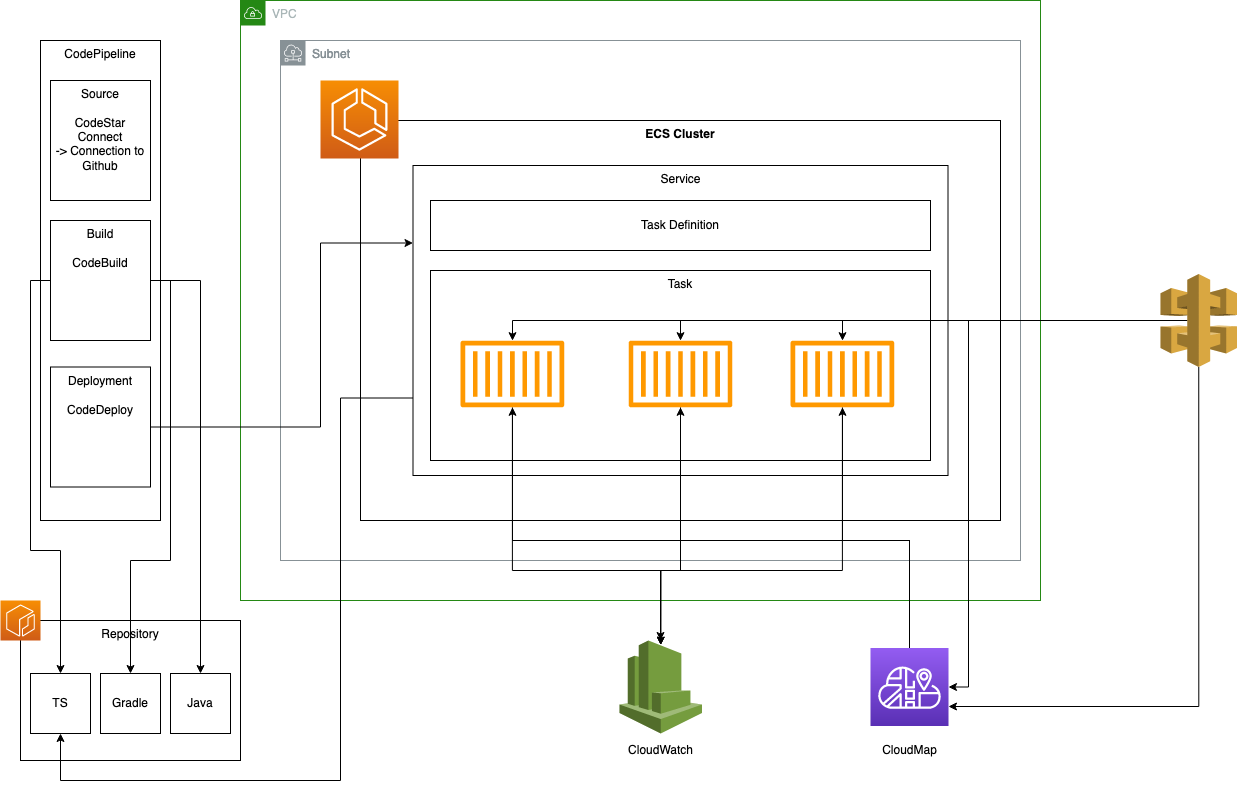
\includegraphics[width=\textwidth]{aws_architecture.png}
    \caption{Architekturentwurf für die AWS-Services}
    \label{fig:CloudArchitektur}
\end{figure}

Die Services werden wir folgt eingesetzt:
\begin{itemize}
    \item \textbf{Code Pipeline} \dots
    \item \textbf{ECS} \dots
    \item \textbf{Code Repository} \dots
\end{itemize}